\chapter{Examples}
\label{chp:examples}

In this chapter we introduce some of the main ideas in iteration theory by
discussing a variety of simple examples. The discussions involve only elementary
mathematics, and our sole objective is to illustrate and stress those features
that will be met in a general context later.

% --- SECTION ------------------------------------------------------------------
% --- INTRODUCTION -------------------------------------------------------------
\section{Introduction}

\begin{proposition}[{$z_n \xrightarrow[n \to \infty]{} w \implies w$ is a fixed
    point}] Let $z_0 \in \ExtC$, $R$ be a rational function in $\ExtC$, and $z_n
    = R^n(z_0)$. Then if $z_n$ converges when $n$ goes to infinity, $\lim_{n \to
    \infty} z_n = w$ is a fixed point of $R$.
\end{proposition}

\begin{proof}
    Since $R$ is continuous (everywhere where it is defined, i.e., the
    denominator is not zero) because it is a rational function, the following is
    true:
    \begin{equation*}
        w = \lim_{n \to \infty} z_n = \lim_{n \to \infty} R(z_{n-1}) = R\left(\lim_{n \to \infty} z_{n-1}\right) = R(w).
    \end{equation*}
    Then, $w = R(w)$, so it is a fixed point.
\end{proof}

\textbf{Intuition:} Let's see why the derivative can work for determining if a
point is attracting or repelling. Since $|R(z) - \zeta| = |R(z) - R(\zeta)|
\simeq |R'(\zeta)| |z - \zeta|$ if $z$ is close enough to $\zeta$, we have that
if $|R'(\zeta)| < 1$, $z_n \to \zeta$, and if $|R'(\zeta)| > 1$, $z_n$ will be
initially repelled from $\zeta$. (A rigorous contradiction proof follows in the
notes ensuring $z_{n+1}$ cannot arbitrarily stay closer than $z_n$ if repelled).

% --- SECTION ------------------------------------------------------------------
% --- ITERATION OF MÖBIUS TRANSFORMATIONS --------------------------------------
\section{Iteration of Möbius Transformations}

\begin{definition}[Möbius Transformation]
    A \emph{Möbius transformation} is a rational function $R: \ExtC \to \ExtC$
    of the form
    \begin{equation*} 
        R(z) = \frac{az+b}{cz+d},
    \end{equation*}
    where $a, b, c, d \in \C$ and $ad - bc \neq 0$.
\end{definition}

\begin{theorem}[Classification of Möbius Transformations]
    Given $R$ a Möbius transformation, then either it has:
    \begin{enumerate}
        \item One fixed point, $\zeta$, and for every $z \in \C$, $R^n(z) \to
        \zeta$.
        \item Two fixed points, $\zeta_1$ and $\zeta_2$, and for every $z \in
        \ExtC$ either:
        \begin{enumerate}
            \item $R^n(z) \to \zeta_1$
            \item $R^n(z) \to \zeta_2$
            \item $R^n(z)$ moves cyclically over a finite set of points.
            \item $\{R^n(z) : n \in \Nzero\}$ forms a dense subset of a circle.
        \end{enumerate}
    \end{enumerate}
\end{theorem}

\begin{proof}
    First, observe that $R$ cannot have $0$ fixed points. Solving $R(z) = z$:
    \begin{equation*}
        \frac{az+b}{cz+d} = z \implies cz^2 + (d-a)z - b = 0
    \end{equation*}
    This is a quadratic equation, so it always has $1$ or $2$ solutions in
    $\ExtC$ (if $c=0$, $\infty$ is a fixed point). 

    \textbf{Case 1: One fixed point.} Suppose the fixed point is $\infty$. Then
    $R(z) = z + \beta$ for some $\beta \in \C$:
    \begin{equation*}
        R(\infty) = \infty \implies c=0 \implies R(z) = \frac{a}{d}z + \frac{b}{d} = \alpha z + \beta.
    \end{equation*}
    We also want $R$ to have no other fixed point:
    \begin{equation*}
        R(z) = z \iff \alpha z + \beta = z \iff (\alpha - 1)z + \beta = 0,
    \end{equation*}
    hence $\beta$ has to be $\neq 0$ (otherwise $z=0$ is a fixed point) and
    $\alpha=1$ (otherwise $z=\beta/(\alpha-1)$ is a fixed point).
    
    If $R$ has a general fixed point $\zeta$, we can define the Möbius
    transformation S by using the conjugation $g(z) = \frac{1}{z-\zeta}$ and $S
    = g \circ R \circ g^{-1}$. Since conjugation preserves the number of fixed
    points, $S$ has exactly one fixed point at $\infty$, meaning $S$ is a
    translation $S(z) = z + \beta$. Thus, $S^n(z) \to \infty$, which implies
    $R^n(z) \to \zeta$.

    \textbf{Case 2: Two fixed points.} Suppose the fixed points are $0$ and
    $\infty$ (it can be shown similarly to the previous case). Then $R(z) = k z$
    for some $k \in \C \setminus \{0, 1\}$. Analyzing $R^n(z) = k^n z$:
    \begin{itemize}
        \item If $|k| < 1$, then $R^n(z) \to 0$.
        \item If $|k| > 1$, then $R^n(z) \to \infty$.
        \item If $|k| = 1$ and $k$ is a root of unity, it cycles over a finite
        set of points.
        \item If $|k| = 1$ and $k$ is not a root of unity, the subset will be
        dense in a circle $|z| = |z_0|$.
    \end{itemize}
    For a general map with two fixed points $\zeta_1, \zeta_2$, we conjugate via
    $g(z) = \frac{z-\zeta_1}{z-\zeta_2}$ to place the fixed points at $0$ and
    $\infty$, yielding the same behavioral classification.
\end{proof}

% --- SECTION ------------------------------------------------------------------
% --- ITERATION OF z^2 ---------------------------------------------------------
\section{Iteration of $z \mapsto z^2$}

\begin{definition}[Forward and Backward Invariant]
    Given a set $E \subseteq \ExtC$ and a rational function $R: \ExtC \to
    \ExtC$, we say $E$ is:
    \begin{enumerate}
        \item \emph{Forward invariant} if $R(E) \subseteq E$.
        \item \emph{Backward invariant} if $R^{-1}(E) \subseteq E$.
    \end{enumerate}
\end{definition}

\begin{definition}[Periodic Point]
    Given a rational function $R: \ExtC \to \ExtC$ and $z \in \ExtC$, we say $z$
    is \emph{periodic with period $k$} if $R^k(z) = z$.
\end{definition}

In the Julia set of $z \mapsto z^2$ (which is $J = \{z : |z| = 1\}$), two close
points may behave radically differently. And it has this properties:
\begin{enumerate}
    \item Given $I$ an arc in $J$, $\exists N \in \Nzero$ such that $\forall n
    \geq N$, $R^n(I) = J$.
    \item $\exists z_0 \in J$ such that $\{R^n(z_0) \mid n \in \Nzero\}$ is
    dense in $J$.
    \item $\exists z_0 \in J$ such that $\{R^n(z_0) \mid n \in \Nzero\}$ is
    finite.
\end{enumerate}

% --- SECTION ------------------------------------------------------------------
% --- TCHEBYCHEV POLYNOMIALS ---------------------------------------------------
\section{Tchebychev Polynomials}
\label{sec:tchebychev_polynomials}

\begin{theorem}[Characterization of Tchebychev polynomials]
    Suppose that $T$ is a polynomial of degree $k$, where $k \geq 2$. Then, the
    interval $[-1, 1]$ is both forward and backward invariant under $T$ if and
    only if $T$ is $T_k$ or $-T_k$.
\end{theorem}
\begin{proof}
    See \cite[11--12]{Beardon1991}
\end{proof}

% --- SECTION ------------------------------------------------------------------
% --- ITERATION OF z^2 - 1 -----------------------------------------------------
\section{Iteration of $z \mapsto z^2 - 1$}
For polynomials like $P(z) = z^2 - 1$, points outside a certain radius escape to
infinity ($z \in F_\infty \implies P^n(z) \to \infty$).

$P(F_0) = F_{-1}$, $P(F_{-1}) = F_0$.

$P(\Omega) \to \ldots, F_0, F_{-1}, F_0, \ldots$, $\Omega$ a Fatou set $\neq
F_\infty$.

% --- SECTION ------------------------------------------------------------------
% --- ITERATION OF z^2 + c -----------------------------------------------------
\section{Iteration of $z \mapsto z^2 + c$}
Recall Vieta's formulas. Given a polynomial $P(x) = ax^2 + bx + c$ with roots
$r_1, r_2$:
\begin{equation*}
    r_1 + r_2 = -\frac{b}{a}, \quad r_1 r_2 = \frac{c}{a}.
\end{equation*}
In general, given a polynomial of degree $n$, $P(x) = a_n x^n + a_{n-1} x^{n-1}
+ \dots + a_1 x + a_0$
\begin{equation*}
    \sum_{i=1}^{n} r_i = -\frac{a_{n-1}}{a_n}, \quad \prod_{i=1}^{n} r_i = (-1)^n \frac{a_0}{a_n},
\end{equation*}
and
\begin{equation*}
    \sum_{1 \le i < j \le n}^{n} r_i r_j = \frac{a_{n-2}}{a_n}, \quad \sum_{1 \le i < j < k \le n}^{n} r_i r_j r_k = \frac{a_{n-3}}{a_n}, \quad \cdots
\end{equation*}

A second degree polynomial can be transformed into a composition of two affine
transformations and $z^2$:
\begin{equation*}
    P(z) = z - z^2 = -(z^2 - z) = -\left(z^2 - z + \frac{1}{4} - \frac{1}{4}\right) = -\left(\left(z - \frac{1}{2}\right)^2 - \frac{1}{4}\right).
\end{equation*}
Then defining
\begin{equation*}
    h(z) = z - \frac{1}{2} \quad , \quad g(z) = z^2 \quad , \quad f(z) = -\left(z - \frac{1}{4}\right) = \frac{1}{4} - z,
\end{equation*}
we have
\begin{equation*}
    P(z) = f \circ g \circ h(z) = f \circ g \left(z - \frac{1}{2}\right) = f \left(\left(z - \frac{1}{2}\right)^2\right) = -\left(\left(z - \frac{1}{2}\right)^2 - \frac{1}{4}\right) = -(z^2 - z).
\end{equation*}

% --- SECTION ------------------------------------------------------------------
% --- ITERATION OF z + 1/z -----------------------------------------------------
\section{Iteration of $z \mapsto z + 1/z$}
We consider the dynamics of the rational map defined by:
\begin{equation*} R(z) = z + \frac{1}{z} \end{equation*}

\subsection*{Real Axis:}
For real values $z = x \in \R$ with $x > 1$:
\begin{equation*}
    R(x) = x + \frac{1}{x} > x.
\end{equation*}
The sequence of iterates increases monotonically towards $+\infty$.

\begin{center}
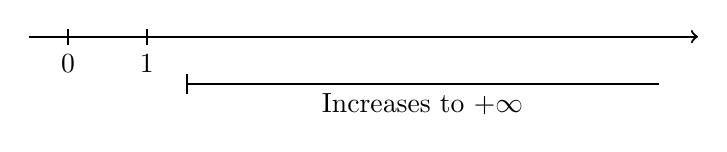
\begin{tikzpicture}
    % Real line
    \draw[{->}, thick] (-0.5,0) -- (8,0);
    % Ticks
    \draw[thick] (0,0.1) -- (0,-0.1) node[below] {$0$}; \draw[thick] (1,0.1) --
    (1,-0.1) node[below] {$1$};
    
    % Dynamics indicator
    \draw[|-, thick] (1.5,-0.6) -- (7.5,-0.6); \draw[thick] (7.5,-0.6) --
    (7.5,-0.6); \node[below] at (4.5,-0.6) {Increases to $+\infty$};
\end{tikzpicture}
\end{center}

\vspace{1em}

\subsection*{Imaginary Axis:}
For purely imaginary values $z = iy \in i\R$ with $y > 1$:
\begin{equation*}
    R(iy) = iy + \frac{1}{iy} = i\left(y - \frac{1}{y}\right).
\end{equation*}
Since $y > 1$, $y - \frac{1}{y} < y$. Thus, the imaginary part decreases towards
$0$ as long as $y > 1$. Once it eventually exits this regime ($y \leq 1$), the
behavior changes completely.

\begin{center}
\begin{tikzpicture}
    % Imaginary line
    \draw[{->}, thick] (0,-0.5) -- (0,4.5);
    % Ticks
    \draw[thick] (0.1,0) -- (-0.1,0) node[left] {$0$}; \draw[thick] (0.1,1) --
    (-0.1,1) node[left] {$1$};
    
    % Range indicator
    \draw[|-|, thick] (0.8,1.2) -- (0.8,4.2); \node[right, text width=8cm] at
    (1.2,2.7) {Decreases to $-\infty$ (when it eventually exits ($y \le 1$)
    behavior changes)};
\end{tikzpicture}
\end{center}

\vspace{1em}

\subsection*{Region $x > 1$:}
In the half-plane where $\text{Re}(z) > 1$, the trajectories flow outwards
towards the right along curves that flatten asymptotically.

\begin{center}
\begin{tikzpicture}
    % Axes
    \draw[{->}, thick] (-0.5,0) -- (4,0); \draw[thick] (0,-1.5) -- (0,1.5);
    
    % Dashed line x = 1
    \draw[dashed, thick] (1,-1.5) -- (1,1.5);
    
    % Flow arrows
    \draw[{->}, >=Stealth, thick] (1.4,1) .. controls (2,0.5) and (2.5,0.2) ..
    (3.2,0.1); \draw[{->}, >=Stealth, thick] (1.6,0.6) .. controls (2.2,0.3) and
    (2.6,0.15) .. (3.3,0.05);
    
    \draw[{->}, >=Stealth, thick] (1.4,-1) .. controls (2,-0.5) and (2.5,-0.2)
    .. (3.2,-0.1); \draw[{->}, >=Stealth, thick] (1.6,-0.6) .. controls
    (2.2,-0.3) and (2.6,-0.15) .. (3.3,-0.05);
\end{tikzpicture}
\end{center}

\vspace{1em}

\subsection*{Analyzing the Conjugate Map:}
We can understand the behavior at infinity by conjugating via $g(z) =
\frac{1}{z}$, which maps the neighborhood of $\infty$ to a neighborhood of the
origin. Let $S = g \circ R \circ g^{-1}$. Since $g^{-1}(z) = \frac{1}{z}$, we
have:
\begin{equation*}
    S(z) = g\left(R\left(\frac{1}{z}\right)\right) = \frac{1}{\frac{1}{z} + z} = \frac{z}{1 + z^2},
\end{equation*}
where $g = \frac{1}{z}$. See
figure~\ref{fig:action_of_z_plus_one_over_z_near_infinity} for the action of $R$
near $\infty$.

\begin{figure}[htbp]
    \centering
    
\includegraphics[width=0.5\textwidth]{beardons_book/action_of_z_plus_one_over_z_near_infinity.png}
    \caption{Action of $z \mapsto z + 1/z$ near $\infty$.}
    \label{fig:action_of_z_plus_one_over_z_near_infinity}
\end{figure}

% --- SECTION ------------------------------------------------------------------
% --- ITERATION OF 2z - 1/z ----------------------------------------------------
\section{Iteration of $z \mapsto 2z - 1/z$}
For $R(z) = 2z - 1/z$, we find the fixed points:
\begin{itemize}
    \item $\zeta_1 = 1$ (repelling),
    \item $\zeta_2 = -1$ (repelling),
    \item $\zeta_3 = \infty$ (attracting).
\end{itemize}

% --- SECTION ------------------------------------------------------------------
% --- NEWTON's APPROXIMATION ---------------------------------------------------
\section{Newton's Approximation}
To find the roots of a polynomial function $f$ in $\R$, the Newton-Raphson
method uses the formula:
\begin{equation*}
    x_{n+1} = x_n - \frac{f(x_n)}{f'(x_n)}.
\end{equation*}
Given $f$ in $\C$, we can define the rational function:
\begin{equation*}
    R(z) = z - \frac{f(z)}{f'(z)}.
\end{equation*}
And the analysis of these kinds of functions (rational functions), falls within
the scope of this text.

Note that, in $\R$ that kind of approximation works, but in $\ExtC\ldots$ the
conditions of $z_0$ to converge to a root are hard and have to do with the Julia
set of $R$ (which for polynomials $f$ with degree $3$ or more is usually a
complex fractal).

Properties of the Newton method:
\begin{enumerate}
    \item The roots of $f$ correspond with fixed points of $R$ (proved in the
    book \cite{Beardon1991}).
    \item Successive iterates of $R$ have a tendency to converge to an
    attracting fixed point of $R$.
\end{enumerate}

Thus, if $\zeta$ is a zero of $f$ which gives rise to an attracting fixed point
of $F$, then,
\begin{equation*}
    z_n = F^n(z_0) \xrightarrow[n \to \infty]{} \zeta
\end{equation*}
for at least initial guesses $z_0$ of $\zeta$ sufficiently accurate.

When $z_0$ is far from $\zeta$ the problem of deciding if $z_n \to \zeta$ is
much harder.

In the book (\cite{Beardon1991}) there is analysis of polynomials of degree $2$
with distinct roots.

A formulation of a theorem for polynomial with real distinct roots: $z_n$
converges to a root of $P$ for essentially every $z_0$ (except from a set with
area $0$)

% --- SECTION ------------------------------------------------------------------
% --- GENERAL REMARKS ----------------------------------------------------------
\section{General Remarks}
For typical rational functions $R$, the extended complex plane $\ExtC$ is
divided into $J$ (Julia set) and $F$ (Fatou set).
\begin{itemize}
    \item $F$ preserves proximity.
    \item $J$ is in every sense chaotic.
    \item $J$ and $F$ are both forward and backward invariant.
\end{itemize}